\documentclass[conference]{IEEEtran}
\usepackage{amsmath,amssymb,amsthm}
\usepackage{graphicx}
\usepackage{booktabs}
\usepackage{url}
\usepackage[hidelinks]{hyperref}
\usepackage{microtype}
\usepackage{xcolor}

\newcommand{\ind}{\mathbf{1}}
\newcommand{\E}{\mathbb{E}}
\newcommand{\Prob}{\mathbb{P}}
\newcommand{\N}{\mathcal{N}}
\newcommand{\dd}{\mathrm{d}}

\title{Hypergraph--Nonlinear--Latency Voter Model:\\
Corrected Semantics and a Reproducible Reassessment}

\author{%
\IEEEauthorblockN{Xinyi Cui, Leyi Yan, Ruiying Cai, Chaowei Xiao}
\IEEEauthorblockA{Group 36}
\thanks{Revised edition of the Group 36 project report \cite{hnl2024}. The original manuscript and the v1 prototype are archived at \url{https://github.com/cxy2696/Hypergraph-Nonlinear-Latency-Voter-Model/tree/v1.0-legacy}. Code, data, result tables, and the run manifest for this version are at \url{https://github.com/cxy2696/Hypergraph-Nonlinear-Latency-Voter-Model}.}
}

\IEEEoverridecommandlockouts
\hypersetup{pdftitle={Hypergraph-Nonlinear-Latency Voter Model: Corrected Semantics and a Reproducible Reassessment},pdfauthor={Xinyi Cui, Leyi Yan, Ruiying Cai, Chaowei Xiao}}
\begin{document}
\maketitle

\begin{abstract}
Group interaction, nonlinear conformity, and heterogeneous reaction delays are three plausible ingredients of opinion dynamics. An earlier project combined them into a hypergraph--nonlinear--latency (HNL) voter model and reported simulations on social-media sentiment data. We rebuilt that model, audited the released code, and reran the experiments under a paired design with 30 replicates per cell. The rebuild exposed two implementation defects and one conceptual one: a data pipeline had mapped every post to the same opinion, the update rule depended on the order of the hyperedge list, and, more consequentially, the absorbing states of the model had been assumed to be global consensus. On a disconnected hypergraph they are component-wise consensus states, so a fragmented graph freezes into a mosaic rather than converging. We fixed the pipeline and the update, made the absorbing structure explicit, and replaced visual comparisons with bootstrap intervals, paired permutation tests, Holm correction, and censoring-aware summaries. Under this design the nonlinearity claim survives: an 80\% majority is reached in none of the runs at $q=0.5$ and in 87--100\% of the runs at $q=2.5$. The latency-variance claim holds only at low $q$, oscillations are damped transients rather than sustained cycles, and larger $q$ produces smaller cascades, not larger ones. On the Kaggle hashtag graph, none of 900 runs reaches 80\%; the largest final majority is 0.754. The durable result is the nonlinear mechanism, not the three-way narrative that originally framed it.
\end{abstract}

\begin{IEEEkeywords}
opinion dynamics, voter model, hypergraph, nonlinear influence, latency, absorbing states, reproducibility
\end{IEEEkeywords}

\section{Introduction}

The voter model is one of the simplest stochastic descriptions of opinion change. Each node carries a binary opinion and, when it updates, copies the opinion of a randomly chosen neighbour. The model has no parameters beyond the interaction structure, and its long-run behaviour is well understood: on a finite connected graph the process reaches unanimity almost surely, while fragmented or infinite structures can sustain coexistence \cite{clifford1973,holley1975,liggett1999}. These properties have made the voter model a standard baseline for consensus, polarisation, and the effect of network structure on collective outcomes \cite{castellano2009,sood2005,baronchelli2018}.

The baseline is also easy to criticise. Real influence is rarely pairwise: people argue in group chats, forums, meetings, and hashtag threads. Adoption is rarely linear: a small local majority may be ignored, while a large one may sweep a group. And reactions are rarely simultaneous: some people answer within minutes, others after days. Each of these observations has generated its own literature, respectively hypergraph voter models \cite{golovin2023}, nonlinear voter models \cite{ramirez2023}, and voter models with latency \cite{palermo2024}. Combining them is a natural next step, and an earlier project did exactly that \cite{hnl2024}. It proposed a hypergraph--nonlinear--latency (HNL) voter model, simulated it on random hypergraphs and on a Kaggle sentiment dataset, and concluded that lower nonlinearity and higher latency variance prolong diversity, that moderate nonlinearity produces sustained oscillations, that higher nonlinearity produces larger cascades, and that the model replicates observed social-media dynamics.

This paper reports what happened when we rebuilt that model and checked those conclusions. The rebuild was not a matter of cleaning up notation. The released code contained a sentiment-mapping bug that assigned the same opinion to every post, a random initialisation step that discarded the data-derived opinions, duplicate node identifiers inside hyperedges, and an update loop whose result depended on the order in which hyperedges happened to be stored. Some of these are ordinary implementation defects. One is more consequential: the model's absorbing states had been assumed to be global consensus, whereas on a disconnected hypergraph they are component-wise consensus states. A fragmented graph therefore does not converge to one opinion; it freezes into a mosaic, and the global majority is set by how the components happen to break. That distinction changes how the dataset results should be read.

We kept the model family and changed the parts that determine what its numbers mean. Section~III gives a precise specification with three aggregation rules: a node-centred mean (the default), a node-centred sample, and the literal edge sweep of the original pseudocode. Section~IV proves the absorbing-state result, derives the mean-field transition at $q=1$, and explains why latency can delay but not sustain an oscillation. Section~V describes a paired design with common random numbers, 30 replicates per cell, and inference that respects censoring. Section~VI reports the results. The short version is that the nonlinear mechanism survives and the other three claims do not: latency variance matters only near balance, the observed oscillations damp, cascades shrink as $q$ grows, and the Kaggle graph cannot support a population-level consensus experiment at all.

The contribution is therefore a correction and a reassessment, not a new model. We make four concrete contributions:
\begin{enumerate}
\item a specification and reference implementation that are order independent and seeded, together with the three update rules needed to compare the original algorithm with the intended node-centred process;
\item a characterisation of the absorbing set of the process, including the $2^{C}$ mosaic count and the implications for fragmented graphs;
\item a paired reanalysis of the original claims, with confidence intervals, effect sizes, and censoring-aware consensus times;
\item a reproducibility package in which every reported number is generated by one command and tied to a commit, a parameter set, and a data hash.
\end{enumerate}
We do not claim that the HNL model is a validated description of social media. The dataset supplies a group structure, not a trajectory, and the paper is explicit about that boundary.

\section{Related Work}

\emph{Voter models.} The voter model was introduced independently by Clifford and Sudbury \cite{clifford1973} and Holley and Liggett \cite{holley1975}; Liggett's monograph \cite{liggett1999} remains the standard reference. On a finite connected graph the only absorbing states are the two consensus states, and the consensus time depends on the graph through the spectral gap and on the initial condition through the density of interfaces. On heterogeneous graphs the ordering kinetics change \cite{sood2005}, and on fragmented graphs different components can settle on different opinions. The last point is usually treated as a technicality; in our setting it becomes the main story.

\emph{Hypergraph interactions.} Hypergraphs encode group interactions that cannot be reduced to pairwise edges without losing information. Golovin et al.\ \cite{golovin2023} study an adaptive voter model on hypergraphs in which group memberships reorganise, and report richer behaviour than the pairwise model, including prolonged minority persistence and transitions in consensus behaviour. Our model keeps the hypergraph fixed. That is a deliberate simplification: it isolates the effect of group structure from the effect of group turnover, and it matches the data we have, where hashtag groups are static over the simulation window.

\emph{Nonlinear adoption.} The nonlinear voter model replaces the linear copy probability with a power of the local share, $p\propto S_1^{q}/(S_0^{q}+S_1^{q})$. Ramirez et al.\ \cite{ramirez2023} analyse the ordering dynamics of this family and show that the exponent controls whether the symmetric state is stable. Our mean-field calculation in Section~IV reproduces the same threshold at $q=1$; the difference is that we are interested in the finite-size and fragmented regimes where the threshold is not the end of the story.

\emph{Latency.} Palermo et al.\ \cite{palermo2024} add a refractory period to the voter model and observe spontaneous opinion swings. Their mechanism is a delayed response that can produce oscillatory transients. Our latency is also a refractory period, but the question we ask is different: whether the oscillations persist, and whether their amplitude depends on the variance of the latency distribution. The answer depends on the absorbing structure, which is why Section~IV treats absorption before discussing oscillations.

\emph{Cascades.} Threshold models \cite{granovetter1978,easley2010} explain how small shocks can propagate when a critical fraction of a group is already convinced. The HNL model measures cascades as the fraction of nodes that change opinion in one sweep, which is a narrower quantity than the threshold-model cascade. We keep the original metric for comparability, and we point out in Section~VI where the interpretation changes because of it.

\section{Model and Semantics}

\subsection{Structure and state}
Let $H=(V,E)$ be a hypergraph with $V=\{1,\dots,n\}$ and hyperedges $e\in E$, $e\subseteq V$, $|e|\ge2$. Each node $i$ has a positive influence weight $\alpha_i>0$ and a binary opinion $X_i(t)\in\{0,1\}$ at sweep $t$. $E_i=\{e\in E:i\in e\}$ is the set of incident hyperedges and $d_i=|E_i|$. Nodes with $d_i=0$ are isolated; they never update and are excluded from the consensus denominator when we analyse the active graph.

For $x\in\{0,1\}$ and $e\in E$, the influence score of opinion $x$ in group $e$ is
\begin{equation}
S_x(e)=\sum_{j\in e}\alpha_j\,\ind[X_j(t)=x].
\label{eq:score}
\end{equation}
The adoption kernel of the group is
\begin{equation}
\pi_e(t)=\frac{S_1(e)^{q}}{S_0(e)^{q}+S_1(e)^{q}},
\label{eq:kernel}
\end{equation}
with $\pi_e=\tfrac12$ when $S_0=S_1=0$. The exponent $q>0$ controls conformity. At $q=1$ the kernel is the weighted share of opinion~1. For $q>1$ it is convex and amplifies a local majority; for $q<1$ it is concave and gives a minority disproportionate weight. In the limits, $\pi_e\to\tfrac12$ as $q\to0^{+}$ when both opinions are present, and $\pi_e\to\ind[S_1>S_0]+\tfrac12\ind[S_1=S_0]$ as $q\to\infty$.

\subsection{From group kernels to a node probability}
A node may belong to several groups with conflicting majorities, so the model needs a rule for combining their kernels. We consider three.

\emph{Node mean (default).} The node averages the kernels of its incident hyperedges:
\begin{equation}
P_i(t)=\frac{1}{d_i}\sum_{e\in E_i}\pi_e(t),\qquad d_i>0.
\label{eq:mean}
\end{equation}
This rule is order independent, uses all the group information available to the node, and reduces to $\pi_e$ when $d_i=1$. It is the rule used in all experiments unless stated otherwise.

\emph{Node sample.} The node draws one incident hyperedge uniformly, $e_i^{\star}\sim\mathrm{Unif}(E_i)$, and sets $P_i(t)=\pi_{e_i^{\star}}(t)$. This rule is also order independent, but it is noisier; it is the closest stochastic analogue of the original code's last-edge-wins behaviour.

\emph{Edge sweep.} The original Algorithm~1 iterates over hyperedges in a fixed order and updates nodes in place. A node may be updated once per incident edge in a sweep, and the last update wins. This rule is order dependent by construction. We keep it for comparison, not as a default; Section~VI shows that the choice is not a numerical detail.

\subsection{Latency and one sweep}
Each node has a latency $L_i\in\mathbb{N}$, drawn once at initialisation, and a clock $T_i(t)$ that records the last sweep at which its opinion changed, with $T_i(0)=0$. Node $i$ is eligible at sweep $t$ when
\begin{equation}
t-T_i(t)\ \ge\ L_i .
\label{eq:eligible}
\end{equation}
For the node-centred rules, all eligible nodes are updated simultaneously from the state at the start of the sweep:
\begin{equation}
X_i(t+1)=
\begin{cases}
\mathrm{Bernoulli}\big(P_i(t)\big), & \text{if eligible and } d_i>0,\\
X_i(t), & \text{otherwise},
\end{cases}
\label{eq:update}
\end{equation}
and $T_i$ is reset to $t$ only when the opinion changes. A node that does not change remains eligible in the next sweep; a node that changes is blocked for $L_i$ sweeps. This is the semantics of the original report and of the reference implementation; it is not the same as resetting the clock after every update attempt, a distinction that matters for event-driven implementations whose scheduling differs.

\subsection{Metrics}
Let $n_x(t)=|\{i:X_i(t)=x\}|$. The paper's three trajectory metrics are
\begin{align}
D(t)&=1-\frac{\max(n_0(t),n_1(t))}{n}, \label{eq:diversity}\\
C(t)&=\frac{1}{n}\sum_{i=1}^{n}\ind[X_i(t)\ne X_i(t-1)], \label{eq:cascade}\\
O&=\mathrm{sd}\big(\bar X(1),\dots,\bar X(T)\big),\qquad
\bar X(t)=\frac1n\sum_i X_i(t). \label{eq:osc}
\end{align}
$D$ is the minority share, $C$ is the fraction of nodes that changed in a sweep, and $O$ is the sample standard deviation of the mean opinion over the observation window. The consensus time $T_c$ is the first $t$ with $\max(n_0,n_1)/n\ge r$, where $r$ is the consensus threshold; runs that do not reach $r$ by the horizon $T$ are right-censored.

For runs that stop before $T$, the terminal state is carried forward and $C$ is set to zero on the padded sweeps; this keeps the window comparable across runs. $O$ mixes genuine oscillation with a monotone trend, so we also report the late/early amplitude ratio
\begin{equation}
\rho=\frac{\mathrm{sd}\big(\bar X(T/2+1),\dots,\bar X(T)\big)}
{\mathrm{sd}\big(\bar X(1),\dots,\bar X(T/2)\big)} .
\label{eq:ratio}
\end{equation}
A stationary oscillation has $\rho\approx1$; a damped transient has $\rho<1$. This is a descriptive diagnostic, not a periodicity test.

\subsection{Relation to the original formulation}
Equations~\eqref{eq:score} and~\eqref{eq:kernel} are the original equations~(1) and~(2). The original equation~(3) wrote the update as an $\arg\max$ over the adoption probabilities, while its Algorithm~1 sampled from those probabilities. We follow the algorithm: the model is a stochastic voter model, and the deterministic $\arg\max$ rule is a separate variant. The original code also differed from both: it computed each edge kernel from the start-of-sweep opinions, wrote into a separate buffer, and let the last incident edge overwrite the node. That is closest to the node-sample rule, not to the in-place edge sweep. We therefore treat the update rule as part of the model specification and report it with every result.

\section{Analytical Results}

\subsection{Absorbing states are component-wise}
The connected components of the hypergraph are the components of its 2-section graph $G_2$, in which $\{i,j\}$ is an edge if some hyperedge contains both $i$ and $j$. Hyperedges never cross components.

\begin{quote}
\textbf{Proposition 1.} Assume $q>0$, $\alpha_i>0$, and $L_i<\infty$. A state $x\in\{0,1\}^{n}$ is absorbing if and only if $x$ is constant on every connected component of $G_2$.
\end{quote}

\begin{proof}
If $x$ is constant on a component, every hyperedge inside it is monochromatic, so $\pi_e\in\{0,1\}$ equals the common opinion. Every eligible node draws its own opinion and nothing changes. Isolated nodes never update.

Conversely, suppose a component is not constant. Choose $i,j$ in it with $x_i\ne x_j$ and a path $i=k_0,\dots,k_\ell=j$ in $G_2$. Some path edge $\{k_{s-1},k_s\}$ has $x_{k_{s-1}}\ne x_{k_s}$; the hyperedge $e$ that witnesses it contains both opinions, so $S_0(e),S_1(e)>0$ and $0<\pi_e<1$. Under the node-mean rule every node of $e$ has $0<P_i<1$; under node sample each has a positive probability of sampling $e$; under the edge sweep the sweep visits $e$ and each eligible node has a positive flip probability. Latencies are finite, so every node becomes eligible infinitely often and the state is not absorbing.
\end{proof}

Two consequences matter for the rest of the paper. First, a hypergraph with $C$ components has exactly $2^{C}$ absorbing states. Global consensus is only two of them. Second, if the graph is connected, Proposition~1 reduces to the classical statement that the only absorbing states are all-0 and all-1, so the process is eventually absorbed in global consensus. If the graph is fragmented, the process is eventually absorbed in a mosaic: each component is internally unanimous, but different components may disagree.

The probability of global consensus on a fragmented graph depends on how the components break. As a reference calculation, if component outcomes were independent with per-component probabilities $p_c$ of choosing opinion~1, then
\begin{equation}
\begin{aligned}
\Prob(\text{global consensus})
&=\prod_{c=1}^{C}p_c+\prod_{c=1}^{C}(1-p_c)\\
&\le \max\!\Big(\prod_c p_c,\prod_c(1-p_c)\Big).
\end{aligned}
\label{eq:mosaic}
\end{equation}
Even with a generous $p_c\in[0.1,0.9]$ for every component, the right-hand side is at most $0.9^{81}\approx2\times10^{-4}$ for the active hashtag graph ($C=81$) and $0.9^{260}\approx1\times10^{-12}$ for the full graph ($C=260$). The components are not independent, so \eqref{eq:mosaic} is not a theorem about the process; it is a scale check. The simulations in Section~VI are consistent with it.

\subsection{Mean-field transition at \texorpdfstring{$q=1$}{q=1}}
Consider a well-mixed population with homogeneous weights and all nodes eligible. Let $\phi_t$ be the fraction of opinion~1. A random edge of size $s$ has $S_1\approx s\phi_t$ and $S_0\approx s(1-\phi_t)$, so
\begin{equation}
\E[\phi_{t+1}\mid\phi_t]\approx f(\phi_t)
=\frac{\phi_t^{q}}{\phi_t^{q}+(1-\phi_t)^{q}} .
\label{eq:meanfield}
\end{equation}
The map has fixed points $0$, $1$, and $\tfrac12$ for $q>0$, and
\begin{equation}
f'\!\left(\tfrac12\right)=q .
\label{eq:derivative}
\end{equation}
The symmetric state is unstable for $q>1$, stable for $q<1$, and neutral for $q=1$. In an infinite well-mixed system this gives a continuous transition at $q=1$: for $q>1$ the population is driven to one of the consensus states, for $q<1$ the interior fixed point is stable, and for $q=1$ the composition performs a neutral diffusion. Finite populations eventually absorb because of demographic noise; the transition describes the drift, not the absorption time. Appendix~A gives the short derivation.

\subsection{Latency changes timing, not the absorbing set}
Eligibility condition~\eqref{eq:eligible} only delays updates. It does not add or remove absorbing states. Since the state space is finite, and from any non-absorbing state a sequence of single-node flips, each with positive probability, can make every component monochromatic, the only recurrent classes are the absorbing mosaics of Proposition~1; the process is therefore absorbed almost surely for any finite latencies. A sustained oscillation would require a non-absorbing recurrent class, which the model does not have. Latency can create a damped wave: when many nodes change, they leave the active pool for a while, which can push the remaining pool the other way. The wave must decay once the components absorb. This is the analytical reason why the original claim of sustained oscillations at moderate $q$ and high latency variance should be treated with suspicion; Section~VI-C checks it empirically.

\section{Experimental Design}

\subsection{Random hypergraphs}
The main experiment uses $n=100$ nodes and $m=200$ hyperedges. Each hyperedge size is drawn uniformly from $\{3,4,5,6\}$ and its members are sampled without replacement. Node weights are drawn from $\N(1,0.2^{2})$ and clipped below at $0.1$. The resulting graph is connected in all replicates, so Proposition~1 predicts global consensus as the only absorbing outcome; the experiment is about how fast it is reached, not whether it is reachable.

\subsection{Parameter grid}
The grid is $q\in\{0.5,1.0,1.5,2.5\}$ and latency $\in$ \{fixed $L=5$, $\N(5,1^{2})$, $\N(5,2^{2})$, $\N(5,4^{2})$, exponential with mean~5\}. The horizon is $T=100$ sweeps, the consensus threshold is $r=0.8$, and each cell has 30 replicates. The update rule is node mean.

\subsection{Paired design and inference}
Each replicate draws one hypergraph, one initial opinion vector, and one vector of uniforms. Latencies for every distribution are obtained from the same uniforms by inverse-CDF sampling, and every $(q,\text{latency})$ cell runs on that replicate. Contrasts are therefore paired: a difference compares the same graph, the same initial condition, and the same latency quantiles. This is a common-random-numbers design, and it removes between-replicate variance from the comparisons.

Uncertainty is reported with percentile bootstrap intervals (2,000 resamples) for means and medians. Paired differences are tested with a two-sided sign-flip permutation test (10,000 permutations), and $p$-values are adjusted with Holm's method within each latency stratum. Effect sizes are reported as Cliff's $\delta$. Consensus times are right-censored at $T$; cells are summarised by the Kaplan--Meier estimator and by the restricted mean survival time
\begin{equation}
\mathrm{RMST}(T)=\int_0^{T}S(u)\,\dd u,
\label{eq:rmst}
\end{equation}
where $S$ is the Kaplan--Meier survival function of ``not yet converged''. RMST is defined even when fewer than half of the runs converge, unlike the median. All analyses are exploratory; the $p$-values are not a family-wise audit of every comparison in the paper.

\subsection{Dataset and preprocessing}
The dataset is the Kaggle \emph{Social Media Sentiments Analysis Dataset} \cite{parmar2024}, released under CC0. It contains 732 posts and 670 unique user identifiers after whitespace normalisation; 617 users appear once, 44 twice, and 9 three times. The file has 191 distinct emotion labels, not the three sentiment classes its name suggests. We map labels to a binary opinion with a documented valence lexicon: 115 labels are positive, 54 negative, and 22 ambiguous. The ambiguous labels are not mapped. At post level this gives 450 positive, 179 negative, and 103 unmapped posts; at user level, 576 users have a mapped opinion in the full graph and 422 in the active graph.

Hyperedges are hashtag groups: the users who used a given hashtag. After normalisation and deduplication, 171 groups of size at least two remain. The full graph has 670 nodes, 260 connected components, and 179 isolated nodes; the largest component has 140 nodes (20.9\%). The active graph removes isolated nodes and has 491 nodes, 81 components, and the same 140-node largest component (28.5\% of the active population). The largest connected component (LCC) has 140 nodes and 45 hyperedges.

We analyse four scopes: full (all 670 users), active (491 users), active with data-derived initial opinions, and the LCC. The first three use 15--30 replicates depending on scope; the LCC uses 15. The random-initialisation runs isolate the effect of graph structure from the effect of the valence mapping; the data-initialised runs show what the mapped sentiments imply.

\subsection{Update-rule sensitivity}
To compare the three aggregation rules, we rerun the random-hypergraph design with node mean, node sample, and edge sweep, using the same replicates (8 per rule and $q$), normal latency with $\sigma=2$, and $T=100$. We also run a long-horizon check on a smaller graph ($n=30$, $m=60$, $q=2.5$, five seeds, up to 20,000 sweeps) to distinguish a slow process from a non-absorbing one.

\subsection{Software and reproducibility}
The experiments use the \texttt{hnl} package in the accompanying repository. Randomness is derived from \texttt{NumPy SeedSequence} streams; no global random state is used. The full suite is regenerated by \texttt{python -m hnl.cli reproduce}, which writes the run tables, the figures, and a manifest containing the git commit, the package versions, the data SHA-256, and the hash of every artifact. The 50 tests cover the kernel, the aggregation rules, the absorbing-state cases, latency gating, the metrics, and the statistical helpers. The original v1 code is preserved at tag \texttt{v1.0-legacy}; it is not modified.

\section{Results}

\subsection{Nonlinearity}
\begin{table*}[t]
\centering
\caption{Cell summaries on random hypergraphs ($n=100$, $m=200$; 30 paired replicates). $P(\mathrm{cons.})$ is the fraction of runs reaching $r=0.8$ within $T=100$; the Kaplan--Meier median $T_c$ is $\infty$ when fewer than half of the runs converge; RMST is in sweeps and equals the horizon when no run converges. $D$, $O$, and $C$ are defined in \eqref{eq:diversity}--\eqref{eq:cascade}.}
\label{tab:random}
\begin{tabular}{@{}lccccccc@{}}
\toprule
Latency & $q$ & $P(\mathrm{cons.})$ & KM $T_c$ & RMST & final $D$ & $O$ & $\max C$ \\
\midrule
fixed & 0.5 & 0.000 & -- & 100.0 & 0.408 & 0.090 & 0.428 \\
 & 1.0 & 0.233 & $\infty$ & 91.4 & 0.368 & 0.111 & 0.391 \\
 & 1.5 & 0.500 & $\infty$ & 78.0 & 0.296 & 0.120 & 0.377 \\
 & 2.5 & 0.867 & 35 & 46.5 & 0.213 & 0.137 & 0.348 \\
\midrule
$\mathcal{N}(5,1^2)$ & 0.5 & 0.000 & -- & 100.0 & 0.448 & 0.077 & 0.276 \\
 & 1.0 & 0.100 & $\infty$ & 97.2 & 0.372 & 0.102 & 0.265 \\
 & 1.5 & 0.400 & $\infty$ & 80.0 & 0.306 & 0.126 & 0.251 \\
 & 2.5 & 0.967 & 41 & 40.1 & 0.187 & 0.133 & 0.235 \\
\midrule
$\mathcal{N}(5,2^2)$ & 0.5 & 0.000 & -- & 100.0 & 0.445 & 0.072 & 0.272 \\
 & 1.0 & 0.067 & $\infty$ & 95.4 & 0.401 & 0.099 & 0.265 \\
 & 1.5 & 0.600 & 93 & 78.5 & 0.261 & 0.126 & 0.247 \\
 & 2.5 & 0.900 & 32 & 41.9 & 0.212 & 0.138 & 0.219 \\
\midrule
$\mathcal{N}(5,4^2)$ & 0.5 & 0.000 & -- & 100.0 & 0.432 & 0.073 & 0.300 \\
 & 1.0 & 0.133 & $\infty$ & 94.6 & 0.383 & 0.090 & 0.289 \\
 & 1.5 & 0.533 & 93 & 69.8 & 0.282 & 0.127 & 0.262 \\
 & 2.5 & 0.967 & 35 & 37.0 & 0.193 & 0.132 & 0.231 \\
\midrule
Exp$(5)$ & 0.5 & 0.000 & -- & 100.0 & 0.462 & 0.068 & 0.335 \\
 & 1.0 & 0.067 & $\infty$ & 97.8 & 0.407 & 0.089 & 0.316 \\
 & 1.5 & 0.500 & $\infty$ & 75.1 & 0.306 & 0.124 & 0.296 \\
 & 2.5 & 1.000 & 21 & 26.0 & 0.180 & 0.110 & 0.244 \\
\bottomrule
\end{tabular}

\end{table*}

\begin{figure*}[t]
\centering
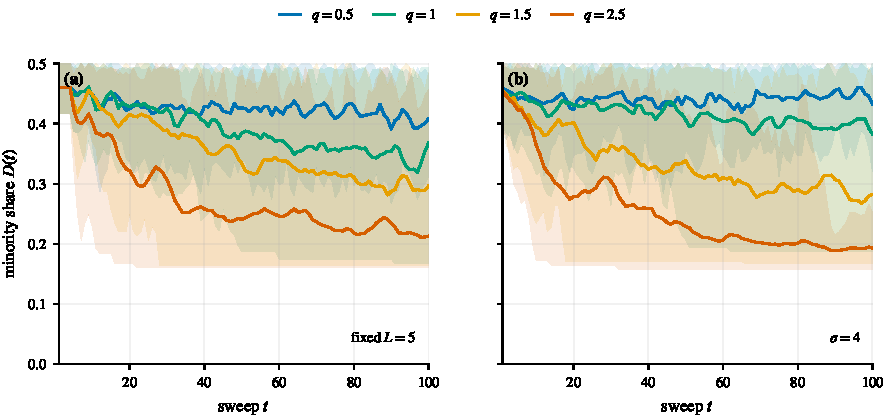
\includegraphics[width=\textwidth]{figures/fig_diversity.pdf}
\caption{Opinion diversity on random hypergraphs. Lines are ensemble means over 30 paired replicates; bands are pointwise 95\% intervals across replicates. (a) Fixed latency $L=5$. (b) Normal latency with $\sigma=4$. Higher $q$ collapses diversity faster in both conditions; the latency change moves the curves only slightly.}
\label{fig:diversity}
\end{figure*}

\begin{figure*}[t]
\centering
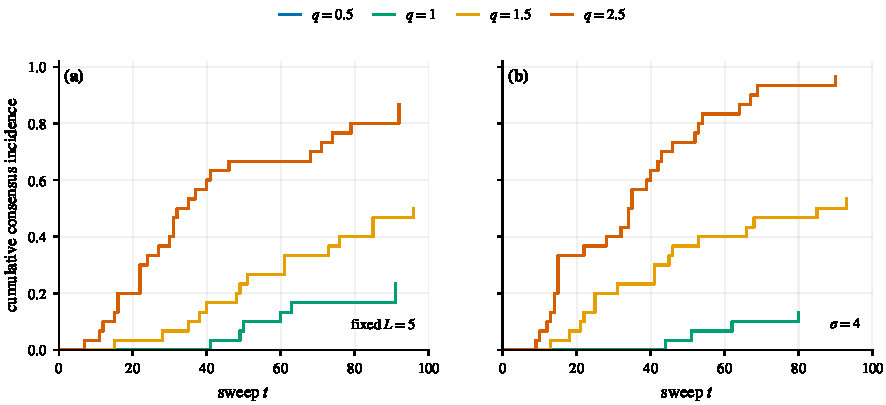
\includegraphics[width=\textwidth]{figures/fig_consensus.pdf}
\caption{Cumulative consensus incidence estimated by Kaplan--Meier. (a) Fixed latency. (b) Normal latency with $\sigma=4$. Curves show the fraction of runs that have reached an 80\% majority by sweep $t$; runs still below the threshold at $T$ are censored. At $q=0.5$ no curve leaves zero; at $q=2.5$ the curves reach 0.87--1.00.}
\label{fig:consensus}
\end{figure*}

Table~\ref{tab:random} and Figs.~\ref{fig:diversity}--\ref{fig:consensus} show the central result. At $q=0.5$ no run in any latency condition reaches 80\% within 100 sweeps. At $q=1.0$ the consensus rate is 6.7--23.3\%, at $q=1.5$ it is 40--60\%, and at $q=2.5$ it is 86.7--100\%. The final minority share falls from 0.408--0.462 at $q=0.5$ to 0.180--0.213 at $q=2.5$. The paired contrast between $q=2.5$ and $q=0.5$ is $-0.195$ to $-0.282$ in final diversity and $+0.867$ to $+1.000$ in consensus probability; all five latency conditions give Holm-adjusted $p=3\times10^{-4}$, the resolution floor of 10,000 permutations with three comparisons, and Cliff's $\delta$ between $0.89$ and $1.00$ (Table~\ref{tab:effects}).

The timing measures tell the same story. The restricted mean time to consensus is at the censoring ceiling (100) for $q=0.5$ and falls to 26--47 sweeps for $q=2.5$. The Kaplan--Meier median is 21--41 sweeps at $q=2.5$; at $q=1.5$ it is resolved only for the two conditions with the largest latency variance (93 sweeps), and at $q=0.5$ it does not resolve at all. The transition is monotone in $q$, and it is large relative to every other factor in the design. This is what the mean-field calculation in Section~IV-B predicts for a connected graph.

\begin{table*}[t]
\centering
\caption{Paired contrasts between $q=2.5$ and $q=0.5$ on random hypergraphs (30 replicates per cell). $\Delta$ is the mean paired difference; intervals are percentile bootstrap 95\% CIs; $p_{\mathrm{Holm}}$ is the Holm-adjusted two-sided sign-flip permutation $p$-value within each latency stratum. The smallest attainable adjusted $p$ is $3\times10^{-4}$.}
\label{tab:effects}
\begin{tabular}{@{}lcccccc@{}}
\toprule
 & \multicolumn{3}{c}{$\Delta$ final diversity} & \multicolumn{3}{c}{$\Delta P(\mathrm{consensus})$} \\
\cmidrule(lr){2-4}\cmidrule(lr){5-7}
Latency & $\Delta$ & 95\% CI & $p_{\mathrm{Holm}}$ & $\Delta$ & 95\% CI & $p_{\mathrm{Holm}}$ \\
\midrule
fixed & -0.195 & [-0.222, -0.166] & $3\times10^{-4}$ & +0.867 & [0.733, 0.967] & $3\times10^{-4}$ \\
$\mathcal{N}(5,1^2)$ & -0.261 & [-0.281, -0.241] & $3\times10^{-4}$ & +0.967 & [0.900, 1.000] & $3\times10^{-4}$ \\
$\mathcal{N}(5,2^2)$ & -0.233 & [-0.262, -0.196] & $3\times10^{-4}$ & +0.900 & [0.767, 1.000] & $3\times10^{-4}$ \\
$\mathcal{N}(5,4^2)$ & -0.239 & [-0.258, -0.219] & $3\times10^{-4}$ & +0.967 & [0.900, 1.000] & $3\times10^{-4}$ \\
Exp$(5)$ & -0.282 & [-0.298, -0.265] & $3\times10^{-4}$ & +1.000 & [1.000, 1.000] & $3\times10^{-4}$ \\
\bottomrule
\end{tabular}

\end{table*}

\subsection{Latency variance}
The latency contrasts are much weaker, and their sign is not stable across $q$. At $q=0.5$, every non-degenerate latency distribution leaves more minority share than fixed latency: $\Delta D=+0.024$ [0.001, 0.046] for $\sigma=4$, $+0.037$ [0.018, 0.058] for $\sigma=2$, $+0.040$ [0.018, 0.063] for $\sigma=1$, and $+0.054$ [0.029, 0.076] for the exponential distribution. The corresponding Holm-adjusted $p$-values are 0.048, 0.006, 0.006, and 0.001. The effect is real but small: it is at most one fifth of the $q$ effect.

At $q=1.5$ there is no detectable latency effect. The $\sigma=4$ contrast is $\Delta D=-0.014$ [$-0.075$, 0.043] and the exponential contrast is $+0.010$ [$-0.056$, 0.079]; both have adjusted $p=1.0$. The intervals exclude effects larger than about 0.08, so the correct statement is not that latency has no effect but that any effect at this $q$ is smaller than the design can resolve. At $q=2.5$ the exponential distribution is associated with less diversity ($\Delta D=-0.033$ [$-0.062$, $-0.009$], $p=0.036$), while $\sigma=4$ gives $-0.020$ [$-0.052$, 0.011], $p=0.50$. Consensus-rate contrasts are all non-significant after Holm; the point estimates at $q=2.5$ are positive for every non-degenerate distribution ($+0.033$ to $+0.133$), which is the opposite of the ``prolongs diversity'' direction but too uncertain to interpret.

The original claim was that high latency variance prolongs diversity. The data support a narrower version: near balance ($q=0.5$), heterogeneous delays slow the decay of the minority by a small amount. At moderate and high $q$ the effect is absent or reversed. Since most of the paper's qualitative discussion concerned $q=1.5$ and $q=2.5$, the general claim does not survive.

\subsection{Oscillations}
\begin{figure*}[t]
\centering
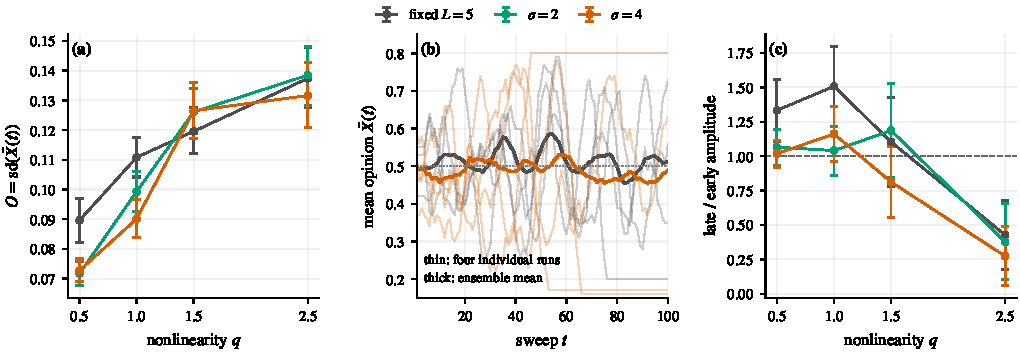
\includegraphics[width=\textwidth]{figures/fig_oscillation.pdf}
\caption{Oscillation diagnostics. (a) $O=\mathrm{sd}(\bar X(t))$ against $q$ for fixed, $\sigma=2$, and $\sigma=4$ latency. (b) Individual mean-opinion trajectories at $q=1.5$; thin lines are four runs, thick lines are ensemble means. (c) Late/early amplitude ratio $\rho$ from \eqref{eq:ratio}; values below one indicate damping. $O$ is higher at $q=2.5$ than at $q=0.5$, and the strongest damping occurs at $q=2.5$, where consensus is reached.}
\label{fig:oscillation}
\end{figure*}

Fig.~\ref{fig:oscillation} summarises the oscillation analysis. $O$ is higher at $q=2.5$ than at $q=0.5$ in every latency condition: the cell means are 0.068--0.090 at $q=0.5$, 0.120--0.127 at $q=1.5$, and 0.110--0.138 at $q=2.5$. The paired contrast at $q=2.5$ against $q=0.5$ is $+0.041$ to $+0.067$, with $p<0.001$ in every latency condition. High latency variance does not increase $O$ at $q=1.5$: the $\sigma=4$ contrast against fixed latency is $+0.007$ [$-0.005$, 0.020], $p=0.885$.

The late/early ratio is more informative. At $q=2.5$ it is 0.11--0.43: the late-window amplitude is a small fraction of the early-window amplitude, which is what a damped transient looks like as consensus is approached. At $q=1.5$ it is 0.81--1.19, and at $q=0.5$ it is 1.02--1.33. The low-$q$ values above one do not indicate a growing oscillation; they reflect slow drift and the fact that the horizon ends before absorption. The intermediate values at $q=1.5$ are consistent with a slow transient over the 100-sweep window, not with a sustained cycle.

This is the empirical counterpart of Proposition~1. The chain is finite and absorbing, so a sustained oscillation is impossible asymptotically. A refractory period can produce a damped wave, and high $q$ makes the wave larger before absorption; it cannot produce a limit cycle. The original claim of sustained oscillations at moderate $q$ and high latency variance is therefore not supported. Part of the discrepancy is methodological: the v1 code plotted the mean opinion, not $O$, so a slow trend could look like a persistent swing.

\subsection{Cascades}
\begin{figure*}[t]
\centering
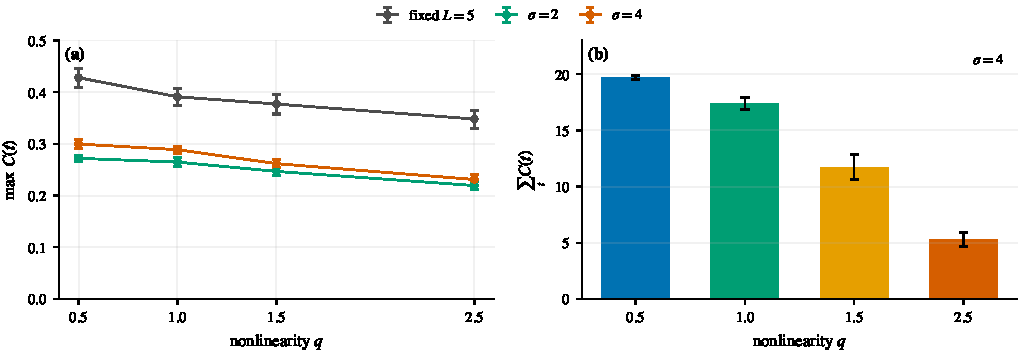
\includegraphics[width=\textwidth]{figures/fig_cascade.pdf}
\caption{Cascade size. (a) Largest single-sweep change, $\max_t C(t)$, against $q$ for fixed, $\sigma=2$, and $\sigma=4$ latency. (b) Summed cascade activity $\sum_t C(t)$ for $\sigma=4$. Both measures decrease with $q$, contrary to the original claim that higher nonlinearity produces larger cascades.}
\label{fig:cascade}
\end{figure*}

The cascade result goes in the opposite direction from the original claim. With fixed latency the largest single-sweep change falls from 0.428 at $q=0.5$ to 0.348 at $q=2.5$; with $\sigma=4$ it falls from 0.300 to 0.231; with $\sigma=2$ it falls from 0.272 to 0.219. The paired contrast at $q=2.5$ against $q=0.5$ is negative in every latency condition ($-0.041$ to $-0.091$), with adjusted $p=3\times10^{-4}$ in all five. Total cascade activity, $\sum_t C(t)$ under $\sigma=4$, falls from 19.7 to 5.3 over the same range.

The mechanism is visible in the diversity trajectories. At low $q$ the population stays near balance, so a single sweep can flip a large fraction of nodes; at high $q$ consensus is reached early, and after that there is little left to flip. The original statement that higher $q$ produces ``more frequent and larger'' cascades is therefore reversed for the paper's own cascade metric. The frequency of changes is indeed higher at low $q$, but the size is also higher; the two do not trade off in the direction the original text assumed.

\subsection{The dataset: a mosaic, not a consensus experiment}
\begin{table*}[t]
\centering
\caption{Dataset results. $C$ is the number of connected components; ``largest'' is the size of the largest component and its share of the scope; $P(\mathrm{cons.})$ is the fraction of runs reaching $r=0.8$; final $D$ is the mean minority share at the horizon; ``max majority'' is the largest final majority observed in any run. The full, active, and data-initialised scopes use 180, 600, and 120 runs, respectively; the LCC uses 180.}
\label{tab:dataset}
\begin{tabular}{@{}lcccccccc@{}}
\toprule
Scope & $n$ & $m$ & $C$ & largest & $P(\mathrm{cons.})$ & final $D$ & max majority \\
\midrule
full & 670 & 171 & 260 & 140 (20.9\%) & 0.000 & 0.463 & 0.613 \\
active & 491 & 171 & 81 & 140 (28.5\%) & 0.000 & 0.449 & 0.754 \\
active, data init & 491 & 171 & 81 & 140 (28.5\%) & 0.000 & 0.383 & 0.743 \\
largest comp. & 140 & 45 & 1 & 140 (100.0\%) & 0.250 & 0.343 & 0.821 \\
\bottomrule
\end{tabular}

\end{table*}

\begin{figure*}[t]
\centering
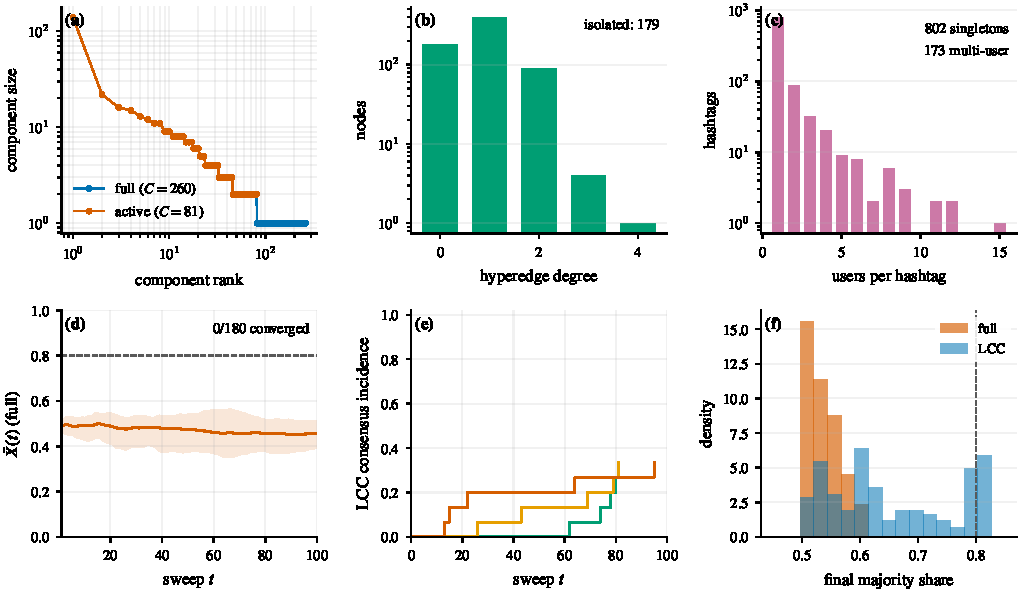
\includegraphics[width=\textwidth]{figures/fig_dataset.pdf}
\caption{The Kaggle hashtag hypergraph. (a) Component-size distributions for the full and active graphs. (b) Degree distribution of the full graph. (c) Distribution of hashtag group sizes; most hashtags are used by one user and create no group. (d) Full-population mean opinion at $q=1.5$, $\sigma=4$; the 80\% threshold is never approached. (e) Consensus incidence of the largest component by $q$. (f) Final majority distributions for the full population and the largest component.}
\label{fig:dataset}
\end{figure*}

Table~\ref{tab:dataset} and Fig.~\ref{fig:dataset} report the dataset analysis. The graph is highly fragmented: 260 components in the full graph and 81 in the active graph; the largest component holds 20.9\% of all users and 28.5\% of the active population. Of 975 distinct hashtags, 802 are used by exactly one user; 173 are multi-user groups, which collapse to 171 unique hyperedges after merging identical groups. The degree distribution is dominated by degree one: the mean degree among covered nodes is 1.20.

Across the 900 population-level runs (600 active, 180 full, 120 data-initialised), the 80\% threshold is never reached. The largest final majority is 0.754 in the active graph, 0.613 in the full graph, and 0.743 with data initialisation. The components nevertheless absorb internally: 97.2\% of active-graph components are unanimous at the end of a run, and 99.1\% in the full graph. This is exactly the mosaic of Proposition~1. The stable diversity in the original figures is an absorbing state, not a dynamical coexistence of opinions.

The largest component is the only scope where consensus is occasionally reachable: 45 of 180 runs (25\%) reach 80\%, and the largest final majority is 0.821. Even there, the graph is sparse (140 nodes, 45 hyperedges, mean degree 1.34), and most runs end below the threshold. The $q$ effect, which dominates the random-hypergraph experiment, is weak at population level: the active-graph contrasts in final diversity lie between $-0.034$ and $+0.009$, and only one of the fifteen contrasts (normal $\sigma=4$, $q=1.5$: $\Delta=-0.034$, $p=0.040$) is significant after Holm. The effect reappears where it should: inside the largest component and in the data-initialised active graph, where higher $q$ lowers final diversity by 0.07--0.17. But even there it does not produce population-wide consensus.

This is the main reason the original ``validation'' claim cannot stand. The dataset has no per-user opinion trajectory; 617 of 670 users appear once, and the model's time index is a sweep, not the timestamp. The hashtag graph supplies a group structure, and that structure turns out to be the dominant fact. A population-level 80\% threshold is not a property of the opinion dynamics on this graph; it is a property of how the components happen to break.

\subsection{Update-rule sensitivity}
\begin{table*}[t]
\centering
\caption{Update-rule sensitivity on random hypergraphs (normal latency, $\sigma=2$; 8 replicates per rule and $q$; $T=100$). The node-centred rules produce the $q$ effect; the literal edge sweep of Algorithm~1 does not reach consensus within the horizon.}
\label{tab:rules}
\begin{tabular}{@{}lcccccc@{}}
\toprule
Rule & $q$ & $P(\mathrm{cons.})$ & RMST & final $D$ & $O$ \\
\midrule
node-mean & 0.5 & 0.000 & 100.0 & 0.438 & 0.091 \\
 & 1.0 & 0.250 & 82.8 & 0.370 & 0.105 \\
 & 1.5 & 0.750 & 52.8 & 0.257 & 0.143 \\
 & 2.5 & 1.000 & 34.1 & 0.179 & 0.120 \\
\midrule
node-sample & 0.5 & 0.000 & 100.0 & 0.431 & 0.078 \\
 & 1.0 & 0.125 & 97.0 & 0.414 & 0.110 \\
 & 1.5 & 0.750 & 63.4 & 0.254 & 0.127 \\
 & 2.5 & 1.000 & 43.8 & 0.184 & 0.141 \\
\midrule
edge sweep & 0.5 & 0.000 & 100.0 & 0.450 & 0.054 \\
 & 1.0 & 0.000 & 100.0 & 0.457 & 0.054 \\
 & 1.5 & 0.000 & 100.0 & 0.456 & 0.055 \\
 & 2.5 & 0.000 & 100.0 & 0.455 & 0.063 \\
\bottomrule
\end{tabular}

\end{table*}

Table~\ref{tab:rules} compares the three aggregation rules on identical replicates. Node mean and node sample agree qualitatively: at $q=2.5$ both reach consensus in all eight runs, and at $q=0.5$ neither does. The edge sweep behaves differently: it reaches consensus in none of the eight runs at any $q$, and its final diversity stays near 0.45. The long-horizon check on a smaller graph ($n=30$, $m=60$, five seeds) shows that the edge sweep is not non-absorbing; it absorbs in 14--146 sweeps, versus 7--36 for node mean and 6--18 for node sample. It is simply much slower at $n=100$.

The mechanism is the interaction between the in-place sweep and the latency clock. A node that changes is blocked for $L_i$ sweeps, but a node that does not change remains eligible and is offered an update on every later incident edge in the same sweep. The last edge then overwrites the result. The net effect reinforces the status quo and slows the approach to consensus. The original code's stale buffer and last-edge-wins rule is closer to node sample than to this in-place sweep, which is consistent with the original figures showing a $q$ effect even though the pseudocode, taken literally, does not.

The practical conclusion is that the update rule is part of the model, not an implementation detail. Results should state which rule was used. We use node mean as the default because it is order independent and reduces to the group kernel when a node has one group. The edge sweep is retained for comparison and for reproducing the original algorithm, not as a recommended default.

\section{Discussion}

\emph{What survives.} The nonlinear mechanism is the durable finding. A convex kernel amplifies local majorities, and on a connected graph this produces a sharp, monotone increase in consensus speed and a matching collapse of diversity. The mean-field transition at $q=1$ is visible in the simulation, and the effect is large enough to survive every reasonable variation in latency and aggregation. If the paper had reported only this result, the correction would be minor.

\emph{Why the latency claim is weaker than it looked.} Latency changes when a node may update, not which states are absorbing. On a connected graph the process absorbs regardless of the latency distribution; latency can only change the path and the time. Near balance, heterogeneous delays slow the decay of the minority a little, because they keep some nodes from reinforcing the emerging majority. Away from balance, consensus is fast and there is little room for the delay distribution to matter. The original claim generalised a low-$q$ effect to the whole parameter range.

\emph{Why the oscillation claim fails.} A finite absorbing chain cannot sustain an oscillation. The observed swings are transients: they are largest when $q$ is high and consensus is being approached quickly, and they damp as the components absorb. The original metric made this harder to see because it plotted the mean opinion rather than its standard deviation. The late/early ratio in Fig.~\ref{fig:oscillation}(c) makes the damping explicit.

\emph{Why cascades shrink.} The cascade metric counts the fraction of nodes that change in one sweep. Low $q$ keeps the population near balance, where large flips are possible; high $q$ reaches consensus early, after which few nodes remain to flip. This is a consequence of the same nonlinearity that speeds consensus, not a separate mechanism.

\emph{Why the dataset result is structural.} On a fragmented graph the absorbing states are mosaics. The global majority is a weighted sum of component outcomes, and the 80\% threshold is reached only if enough components happen to choose the same colour. The hashtag graph has 260 components, 179 isolated nodes, and a largest component of 140 nodes; it is not a population in which a global consensus experiment is meaningful. The correct analysis is component-level: which groups freeze, how quickly, and whether the freeze is biased by the initial sentiment. We report the component-absorption rate and the largest-component behaviour for that reason.

\emph{Implications for practice.} If a graph is fragmented, a population-level consensus target will mislead. A practitioner should either analyse the components separately, restrict the target to a connected component, or add bridging interactions and model them explicitly. The same caveat applies to the service implementation that grew out of this model: global ``absorbing'' and ``runaway'' labels are population-level summaries and should be read with the component structure in hand.

\section{Limitations}

The reanalysis has a bounded design. It uses one random-graph family ($n=100$, $m=200$, sizes 3--6), a coarse $q$ grid, a fixed mean latency of five sweeps, and a horizon of 100 sweeps. Thirty replicates give useful intervals for the large $q$ effect but limited power for latency effects of order 0.05; the null results at $q=1.5$ mean ``no effect larger than about 0.08 was detected'', not ``the effect is exactly zero''. The analyses are exploratory and the Holm correction is applied within latency strata, not across the whole paper. A different graph family, a different horizon, or a different latency mean could change the balance between nonlinearity and delay.

The dataset analysis is limited by the data. The file has 732 posts and 670 identifiers, 617 of which appear once; it has no per-user trajectory. The 191 emotion labels are not a stance scale, and the valence mapping is a documented modelling choice rather than a gold standard: 22 labels are ambiguous and excluded, and a different lexicon would move the initial balance. The platform field is pooled, and the handles are pseudonymous. The dataset can support a structural application; it cannot validate a dynamical model.

The model itself is static and binary. It has no edge rewiring, no external shocks, no media or recommendation effects, and no heterogeneous susceptibility beyond the global $q$. Node weights are fixed. Self-influence is included, as in the original score, which gives the process inertia; removing it would change the transient but not the absorbing set. Latency is measured in sweeps, not in wall-clock time. These are modelling choices, not defects, but they bound the claims.

Finally, the update rule is a choice. Node mean is order independent and is the default, but it is not the only defensible aggregation. Node sample gives similar qualitative results with more noise, and the edge sweep gives a much slower process. The paper's conclusions about $q$ are stable across the two node-centred rules; the conclusions about the edge sweep are specific to that rule.

\emph{Availability.} The code is released under the MIT licence and the dataset under CC0. The repository contains the package, the 50 tests, the dataset, the result CSVs, the figure scripts, and the LaTeX source of this paper. The v1 prototype and the original manuscript are preserved at tag \texttt{v1.0-legacy}. The full experiment is regenerated by \texttt{python -m hnl.cli reproduce --root .}; the run manifest records the commit, the package versions, the data SHA-256, and the hash of every artifact.

\section{Conclusion}

The HNL voter model is worth keeping, but its original narrative needs pruning. The nonlinear mechanism is real and large: on connected random hypergraphs, an 80\% majority is reached in none of the runs at $q=0.5$ and in 87--100\% at $q=2.5$. The latency-variance claim survives only near balance and with a small effect. The oscillation claim is incompatible with the absorbing structure of the model, and the cascade claim has the wrong sign for the paper's own metric. On the Kaggle hashtag graph, fragmentation dominates: the process freezes into a component-wise mosaic, and none of 900 runs reaches the global threshold.

The broader lesson is that the absorbing structure of a voter-type model should be established before its transient behaviour is interpreted. On a connected graph, global consensus is the only absorbing outcome and the interesting question is how fast it is reached. On a fragmented graph, the interesting question is which components freeze, and a population-level consensus threshold can be misleading. The revised code, the paired experiments, the full tables, and the run manifest are released with this paper so that the numbers can be checked and the analysis extended.

\appendices
\section{Mean-field derivation}
Let $\phi_t$ be the fraction of opinion~1 in a well-mixed population with homogeneous weights and all nodes eligible. For a random edge of size $s$, the expected scores are $S_1\approx s\phi_t$ and $S_0\approx s(1-\phi_t)$, so the kernel is
\begin{equation}
\pi\approx\frac{(s\phi_t)^{q}}{(s\phi_t)^{q}+(s(1-\phi_t))^{q}}
=\frac{\phi_t^{q}}{\phi_t^{q}+(1-\phi_t)^{q}}=f(\phi_t).
\end{equation}
If every node updates, the expected next fraction is $f(\phi_t)$ up to $O(1/n)$ sampling noise. The fixed points solve $f(\phi)=\phi$. Besides $0$ and $1$, $\phi=\tfrac12$ is a solution for every $q>0$. Differentiating,
\begin{equation}
f'(\phi)=\frac{q\,\phi^{q-1}(1-\phi)^{q-1}}{(\phi^{q}+(1-\phi)^{q})^{2}},
\end{equation}
and at $\phi=\tfrac12$ this is $q$. The symmetric state is therefore unstable for $q>1$ and stable for $q<1$. The derivative formula also shows why the $q<1$ case is delicate near the boundary: as $\phi\to0$, $f'(\phi)\sim q\,\phi^{q-1}\to\infty$, so a tiny minority has a large local pull even though the interior fixed point is stable.

\section{Dataset mapping and structural details}
The valence lexicon assigns 115 of the 191 normalised labels to positive, 54 to negative, and 22 to ambiguous. The ambiguous set includes labels such as \emph{Bittersweet}, \emph{Nostalgia}, \emph{Neutral}, and \emph{Solitude}. Users whose posts are all ambiguous are filled from the empirical positive share when data initialisation is requested; the number of such users is recorded in the manifest. The full graph contains 670 nodes and 171 hyperedges; the active graph contains 491 nodes and the same 171 hyperedges. The largest component contains 140 nodes and 45 hyperedges. The random graphs use the same edge-size range and weight distribution as the original prototype, so the comparison with the original figures is as close as the corrected semantics allow.

\section{Reproducibility}
The repository contains the package, the 50 tests, the dataset, the result CSVs, the figure scripts, and the LaTeX source of this paper. The full experiment is regenerated by
\begin{center}
\texttt{python -m hnl.cli reproduce --root .}
\end{center}
which writes the tables and figures in about 30 seconds on an Apple-silicon laptop and records the commit, the package versions, the data SHA-256, and the artifact hashes in \texttt{results/manifest.json}. The random seeds are fixed; the paired design is described in Section~V-C. The v1 prototype and the original manuscript are preserved at tag \texttt{v1.0-legacy}.

\bibliographystyle{IEEEtran}
\bibliography{refs}

\end{document}
